\setcounter{page}{7}

\pagestyle{fancy}
\fancyhf{}
\fancyhead[L]{\thepage}
\fancyhead[C]{КВАНТ \textperiodcentered{} 1995/\textnumero{}4}
\renewcommand{\headrulewidth}{0pt}


\vspace*{-3.5\baselineskip}
\begin{multicols}{3}
\noindent или, наконец, \[l_{AC}+l_{A_1C} < \frac{2}{3}AA_1 + \frac{1}{3}LL_1 \]

Умножив полученное неравенство на n, мы и получим неравенство (1). 
\vspace{8pt} \hrule \vspace{1pt} \noindent
\parbox{0.85\linewidth}{\large\bfseries\sffamily{Дальнейшее\\ исследование оcновного неравенства}}
\hrule \vspace{8pt}\noindent Нами установлено, что число \(\pi\) лежит в первой трети интервала \((p_n, q_n.)\) при всех \(n\geq 3\). Для того чтобы уточнить расположение числа в этом новом интервале, рассмотрим отношение длин интервалов \((p_n, \pi)\) и \((p, q_n)\). Вычисления показывают (см. таблицы 1, 2), что это отношение длин, т.е. значения дробей \[(q_n - \pi)/(\pi - p_n), n = 3, 6, 12, 24,\] достаточно близки к 2. На основании этих вычислений мы с большой степенью уверенности можем предположить, что в действительности имеет место соотношение 
\begin{equation}
    \lim\limits_{x \to \infty}\frac{q_n - \pi}{\pi - p_n} = 2
\end{equation} 

Для доказательства соотношения (5) заметим, что (рис.9) \[p_n  = n \cdot \sin\frac{\pi}{n}, q_n = n \cdot \tg\frac{\pi}{n}, n\geq3,\] и, следовательно,\[\frac{q_n - \pi}{\pi - p_n} = \frac{1}{\cos\frac{\pi}{n}} \cdot \frac{n\sin\frac{\pi}{n} - \pi\cos\frac{\pi}{n}}{\pi-n\sin\frac{\pi}{n}}.\]

Для анализа полученного выражения нам понадобятся неравенства \[x - \frac{x^3}{6}< \sin{x} < x-\frac{x^3}{6}+\frac{x^5}{120},\]
\begin{equation}
    x > 0,
\end{equation}
значельно улучшающие известное не-
\begin{table}[H] % расположение прямо по месту
    \caption{} 
    \begin{tabularx}{\linewidth} { 
  | >{\centering\arraybackslash}X 
  | >{\centering\arraybackslash}X 
  | >{\centering\arraybackslash}X | } 
    \hline n & p_n & q_n \\ \hline
    3 & 2,59807621 & 5,19615242 \\ 
    6 & 3,00000000 & 3,46410161 \\ 
    12 & 3,10582854 & 3,21539030 \\ 
    24 & 3,13262861 & 3,15965994 \\ 
    48 & 3,13935020 & 3,14608621 \\ 
    96 & 3,14103195 & 3,14271459 \\ 
    192 & 3,14145247 & 3,14187304 \\ 
    384 & 3,14158389 & 3,14166274 \\ 
    768 & 3,14158389 & 3,14161017 \\ 
    1536 & 3,14159046 & 3,14159703 \\ 
    3072 & 3,14159210 & 3,14159374 \\ \hline
    \end{tabularx} % закончили ввод данных таблицы
\end{table} % закрыли таблицу
\begin{figure}[H]
    \centering
    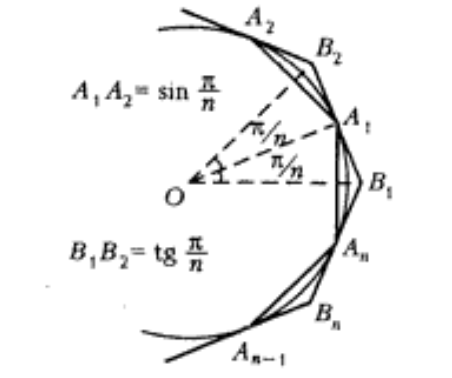
\includegraphics[width=\linewidth]{Рис.9.png}
    \caption*{Рис. 9}
\end{figure} 
\noindent равенство \(\sin{x} < x\) при х>0. Чтобы доказать левое неравенство в (6), положим \[f(x) = \sin{x}-x+\frac{x^3}{6}.\] Тогда имеем \[g_1(x) = f'(x)= \cos{x} - 1 + \frac{x^2}{2},\]\[g_2(x) = g_2'(x)= -\sin{x} + x.\]
Так как \(\sin{x}<x\) при x>0, получим \(g_2(x) > 0\) при x>0. Тем самым функция \(g_1(x)\) возрастает при x>0. Но \(g_1(0) = 0\) и, следовательно, \(g_1(x)>0\) при x>0. Функция \(g_1(x)\) является производной для функции f(x), для которой также f(0)=0. Но при x>0 имеем \(g_1(x)>0\), поэтому функция f(x) также возрастает, следовательно, принимает только положительные значения, т.е. f(x)> 0 при х>0, что и утверждалось.

Аналогично устанавливается правая часть неравенства (6), а также неравенства \[1-\frac{x^2}{2}<\cos{x}<1-\frac{x^2}{2}+\frac{x^4}{24},\]
\begin{equation}
    x > 0.
\end{equation}
(Докажите их самостоятельно!)
\begin{table}[H] % расположение прямо по месту
    \caption{}
    \begin{tabularx}{\linewidth}{ 
  | >{\centering\arraybackslash}X 
  | >{\centering\arraybackslash}X| }  
    \hline n & \((q_n - \pi)/(\pi - p_n)\) \\ \hline
    3 & 3,78012440 \\ 
    6 & 2,27772383 \\ 
    12 & 2,06345553 \\ 
    24 & 2,01552959 \\
    48 & 2,00386204 \\ 
    96 & 2,00096424 \\
    192 & 2,00024098 \\ 
    384 & 2,0006024 \\ 
    768 & 2,0000150 \\ 
    1536 & 2,00000376 \\ 
    3072 & 2,00000094 \\ \hline
    \end{tabularx} % закончили ввод данных таблицы
\end{table} % закрыли таблицу
Из неравенств (6) и (7) вытекают следующие приближенные формулы: \[\sin\frac{\pi}{n}\approx\frac{\pi}{n}-\frac{\pi^3}{6n^3}, \cos\frac{\pi}{n}\approx 1-\frac{\pi^2}{2n^2}.\]
Следовательно, \[\frac{q_n-\pi}{\pi-p_n}=2\cdot(1-\frac{\pi^2}{2n^2})^-1.\]
Что и завершает доказательство соотношения (5), так как \(\frac{\pi^2}{2n^2}\)стремится к нулю при \(n \to \infty\).

Равенство (5) позволяет сделать следующий качественный вывод: число \(\pi\), находясь при любом \(n\geq3\) в интервале \((p_n, \frac{2}{3}p_n+\frac{1}{3}q_n,)\), при всех достаточно большших значениях n ближе к правому концу этого интервала,чем к левому.
\vspace{8pt} \hrule \vspace{1pt} \noindent
\parbox{0.85\linewidth}{\large\bfseries\sffamilyФормула Гюйгенса\\ и ее эффективность} 
\hrule \vspace{8pt}
\noindentАрхимед использовал для вычисления числа \(\pi\) приближенную формулу \(\pi\approx p_n, n\geq3\).

Гюйгенс в своей работе, в частности, получил другую приближенную формулу \(\pi\approx\frac{2}{3}p_n+\frac{1}{3}q_n, n\geq3\), т.е. взял в качестве приближения для числа \(\pi\) правую часть неравенства (1).

Большую эффективность формулы Гюйгенса по сравнению с формулой Архимеда можно обнаружить непосредственными вычислениями на микрокалькуляторе (см.табл.1,3). Отметим, что провести такие вычисления - увлекательная и непростая задача.

Можно сравнить эффективность формул Архимеда и Гюйгенса другим методом, не производя конкретных вычислений для \(р_n\) и \(q_n\). Можно использовать так называемые априорные оценки для точности этих формул, т.е. такие неравенства, которые позво-
\begin{table}[H] % расположение прямо по месту
    \caption{}
    \begin{tabularx}{\linewidth}{ 
  | >{\centering\arraybackslash}X 
  | >{\centering\arraybackslash}X| } 
    \hline n & \(\frac{2}{3}p_n+\frac{1}{3}q_n\) \\ \hline
    3 & 3,464101615137 \\ 
    6 & 3,154700538379 \\ 
    12 & 3,142349130544 \\ 
    24 & 3,141639056219 \\ 
    48 & 3,141595540408 \\ 
    96 & 3,14159283380 \\ 
    192 & 3,141592664850 \\ 
    384 & 3,141592654293 \\ 
    768 & 3,141592653633 \\ 
    1536 & 3,141592653592 \\ 
    3072 & 3,141592653589 \\ \hline
    \end{tabularx} % закончили ввод данных таблицы
\end{table} % закрыли таблицу
\end{multicols}